\chapter{Discussion}


At this point, we studied the state-of-the-art, compared few architectures and selected the best one for aerial views. We also tried to improve our results by using data augmentation, deep transfer learning methods, and compressed ensembles. But even considering all of these experiments, the accuracy of our model is still not perfect, we will propose, in this part, few hints that may improve it.


\section{The architecture}
The selected architecture is the ResNet-152 architecture, with the upscaling method from FCN-16. The figure~\ref{fig:part5:fcn16_resnet_architecture} shows its variant with only 50 layers (for the visibility). It has three really notable characteristics : (1) its depth, it is currently one of the architecture with the biggest number of layers, (2) its residual dimension from ResNet, it permits it to dramatically reduces its number of parameters and so, its computational needs and accuracy, and (3) its end-to-end upscaling method, that can be added at the end of any architecture.

\begin{figure}[ht!]
  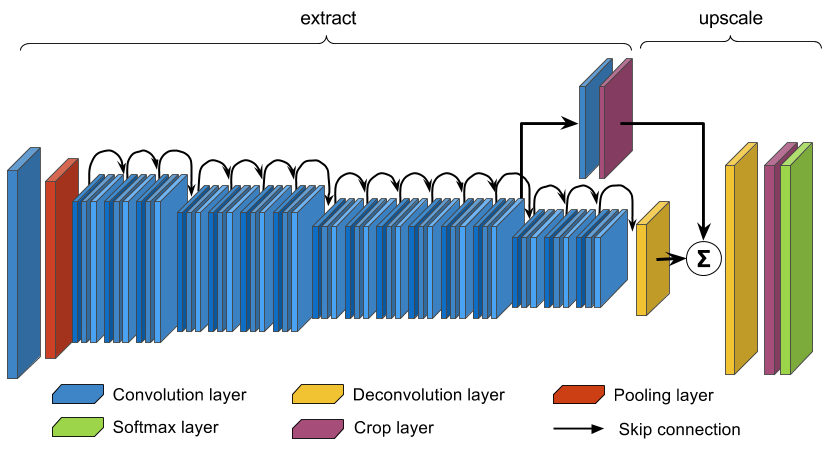
\includegraphics[width=\linewidth,center]{images/part5/fcn16_resnet_architecture.png}
  \caption{Architecture of FCN-16-ResNet-50}\textbf{
  \label{fig:part5:fcn16_resnet_architecture}}
\end{figure}

The results found in section~\ref{4:setups} proves the efficiency of this architecture, but we still can look for a way to improve it. Few points can be considered :
\begin{itemize}
\item About the depth, as we saw in section~\ref{1:comparison:comparison} last architectures seem to reveal that the more deep it is, the best it is. The only problem seems to come from the number of parameters that a deep architecture involves. But for now, the relation between depth and efficiency is not proven yet : the last architecture from Google is actually not as deep as ResNet (75 layers instead of 152) and provides a slight improvement on ILSVRC challenge.
\item We decided to use the ResNet architecture (which provides the best results on ILSVRC 2015 challenge) with its residual connections. However, it is not proven that these connections are the best way to decrease the total number of parameters. Indeed, Google also proposed its own method, involving inception layers. We may have to try to use them in our aerial views, they may be more efficient.
\item We used the upscaling method from FCN-32 and, then, from FCN-16, that improves the accuracy. We tried, at the really beginning of the project, to create the FCN-8-ResNet-x architecture, and it did not improves the accuracy at this moment. Today, we have a better knowledge on the Deep Learning architectures, and maybe we would be able to implement it "the good way", that would improve our results. Also, we did not really studied the upscaling method from SegNet because it is complicated to implement (not included in the last Caffe version, so we need to re-code the upsampling layers by ourself, which is doable, but not considering the given time for this project). This other upsampling method seemed to give better results than FCN-8 according to its authors and combining it with the residual dimension of ResNet may be interesting.
\end{itemize}



\section{Another DTL method ?}
As we saw, our Deep Transfer Learning was not really efficient for improving a learning : it only permits to merge two knowledges from two datasets into a single one. So, our initial expectation is not reached, and that is a bit disappointed because we also did the same experiment using two different datasets (Pascal VOC and MS COCO) and get better results (results displayed in appendices \todo{add ref}).

Considering this, we can imagine that we may be able to improve our learning by modifying some extra-parameters, like decreasing the learning rate through the cycles of the multi-source process, to reduce progressively the influence of the learnings cycle after cycle.



\section{Post-processing, thinking with videos}
An other idea, that we did not explore at all, would be to process images as part of a video instead of single images, all independent. Indeed, the architectures we saw proved their accuracy \textit{via} computer vision challenges, so they need to focus their segmentation skills on single images. But in our case, we know that we are going to process videos, so we can imagine a new architecture that pre-estimate the output segmentation using the one from the previous image (or images). Indeed, using the few earlier images, it is possible to build trivial object tracking and, then, to improve dramatically the accuracy of a system while applying some pre-probabilities on each pixel of next images. This can be done with multiple technical such as Gaussian numbers, or Bayesian optimization.

Using this kind of implementations, we can expect a significant improvement of the accuracy that may allow us to reduce the complexity of our network. It means that, considering the fact that our accuracy will be corrected by our probabilistic-"tracking" method, we can reduce the complexity of the network by reducing its depth, number of parameters, etc.



\section{Possible applications}
Many applications that would need a semantic segmentation on aerial views are possible and, even if we would not implement any of them in this project, we would list here some possibilities :
\begin{itemize}
\item Suspicious traffic or crowd detection : while flying above a city, a drone can determine if the traffic seems suspicious in comparison with his daily experiences (detection of traffic-jams for example, or manifestations, crowds).
\item Pre-cartography : by knowing what it sees (roads, building, etc), a drone can build a map while flying. Of course, it would only be a first draft, but it can provide a good first idea.
\item Creation of a Dynamic map : as a more ambitious project, we can imagine a drone fleet updating, in real time, a map with its intrinsic information, such as traffic, constructions, works ongoing, special events, ...
\item Intelligent vision for rescue or exploration situation : in an urgent exploration mission, a drone may be able to fly above a dangerous area (post-fire, post-crumbling, ...) and detect irregularities such as human bodies to rescue.
\item Intelligent and flexible delivery by drone : nowadays, drones are able to fly from a point A to B, even with difficult weather conditions or ground irregularities. It can be used for drone deliveries, but, for now, the drone would not be able to fly directly to the message addressee : it would go exactly to the given GPS position. Semantic segmentation may be able to fix this and provide delivery hands to hands.
\end{itemize}



